
\appendix
\renewcommand{\thechapter}{\Alph{chapter}}
\renewcommand{\thesection}{\Alph{section}}

\phantomsection
\addcontentsline{toc}{chapter}{Anhang}
\chapter*{Anhang}

\section{Checkliste zur Durchführung der Hauptstudie}
\label{app:checkliste-hauptstudie}

\begingroup
\renewcommand{\arraystretch}{1.5}
\noindent
\begin{tabularx}{\textwidth}{|p{0.6cm}|Y|}
\hline
 & Nummernausgabe \\ \hline
 & Durchführung Fragebogen 1 \\ \hline
 & Github Account erstellen/öffnen $\rightarrow$ Repo auf Github forken
   $\rightarrow$ Github codespaces erklären \\ \hline
 & Gruppe AI: ChatGPT öffnen \\ \hline
 & Gruppe Web Suche: DuckDuckGo $\rightarrow$ show assistant NEVER \\ \hline
 & Garden Simulator erklären \\ \hline
 & Screen recording einrichten \\ \hline
 & Arbeitsaufträge durchgehen \\ \hline
 & Test-Framework durchgehen \\ \hline
 & Start der Ausarbeitung \\ \hline
 & Durchführung Fragebogen 2 \\ \hline
 & Code einsammeln \\ \hline
 & Recording einsammeln \\ \hline
\end{tabularx}
\endgroup

\clearpage
\section{Vorlage der Zuordnungstabelle}
\label{app:zuordnungstabelle}

\begingroup
\small
\renewcommand{\arraystretch}{1.8}
\noindent
\begin{tabularx}{\textwidth}{|>{\centering\arraybackslash}m{1.7cm}|Y|Y|>{\raggedright\arraybackslash}p{1.4cm}|>{\raggedright\arraybackslash}p{2.6cm}|}
\hline
\textbf{Nummer} & \textbf{Vorname} & \textbf{Nachname} & \textbf{Gender (m/w/d)} & \textbf{Geburtsdatum} \\ \hline
1 & & & & \\ \hline
2 & & & & \\ \hline
3 & & & & \\ \hline
4 & & & & \\ \hline
5 & & & & \\ \hline
6 & & & & \\ \hline
7 & & & & \\ \hline
8 & & & & \\ \hline
9 & & & & \\ \hline
10 & & & & \\ \hline
\end{tabularx}
\par
\endgroup

\clearpage
\section{Padlet-Leinwand zur Durchführung der Hauptstudie}
\label{app:padlet}

\begin{center}
  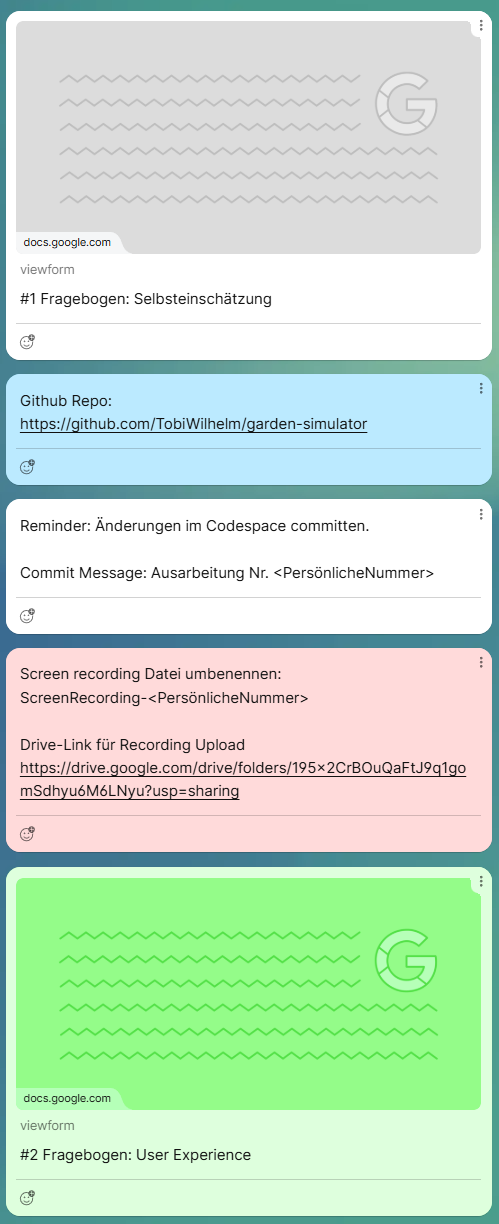
\includegraphics[
    width=\textwidth,
    height=0.95\textheight,
    keepaspectratio
  ]{00_figures/padlet.png}
\end{center}
